\section{来歴}
福岡市立和白東小学校、福岡市立和白丘中学校、福岡工業大学附属高等学校(現・福岡工業大学附属城東高等学校)を卒業\cite{wiki}。

学生時代から筋肉質な体格だったが、当時はボディビルよりもバスケットボールに熱中していた。高校時代に香椎のLBGYMで筋トレを始める。

タレントになった後、福岡の民放番組で2005年と2020年にそのLBGYMを来訪。その様子がRKB毎日放送とTNCテレビ西日本で放映された。

高校時代の同級生には女子柔道家でシドニーオリンピック銅メダリストの日下部基栄がいる。

高校卒業後は吉本総合芸能学院 (NSC) 大阪校に22期生として入学する[2][5]。なお、入学前に1998年10月30日放送の朝日放送テレビ『探偵!ナイトスクープ』の依頼「世界一指を早く回せる男」に出演している[注 1][注 2]。これはバスケットボール選手が指を回す際の仕草である。NSCの同期には、スーパーマラドーナ・久保田かずのぶ(とろサーモン)・キングコングなどがいる。

\begin{figure}[htbp]
  \centering
  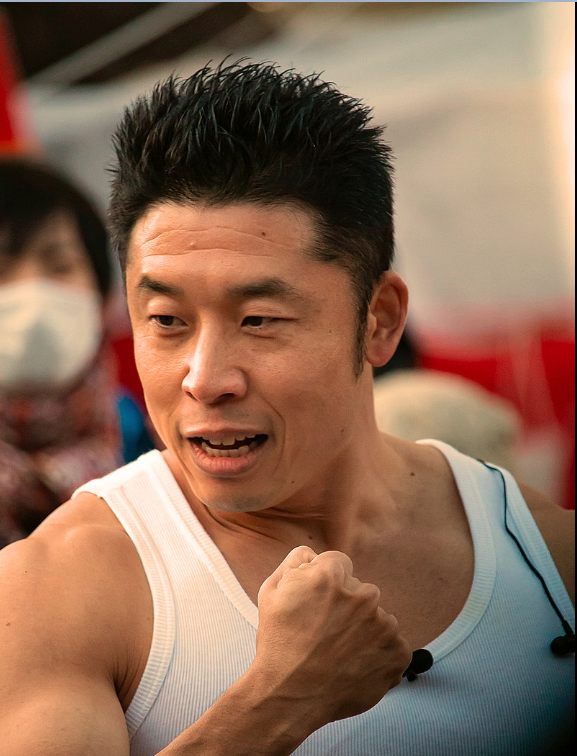
\includegraphics[width=0.5\textwidth]{Chapter1/figures/image.png}
  \caption{キャプテン☆ヒーロー}
  \label{fig:my_label}
\end{figure}
